\documentclass{article}

% if you need to pass options to natbib, use, e.g.:
% \PassOptionsToPackage{numbers, compress}{natbib}
% before loading nips_2018

% ready for submission
\usepackage{nips_2018}

\usepackage{subfiles}

% to compile a preprint version, e.g., for submission to arXiv, add
% add the [preprint] option:
% \usepackage[preprint]{nips_2018}

% to compile a camera-ready version, add the [final] option, e.g.:
% \usepackage[final]{nips_2018}

% to avoid loading the natbib package, add option nonatbib:
% \usepackage[nonatbib]{nips_2018}

\usepackage[utf8]{inputenc} % allow utf-8 input
\usepackage[T1]{fontenc}    % use 8-bit T1 fonts
\usepackage{hyperref}       % hyperlinks
\usepackage{url}            % simple URL typesetting
\usepackage{booktabs}       % professional-quality tables
\usepackage{amsfonts}       % blackboard math symbols
\usepackage{nicefrac}       % compact symbols for 1/2, etc.
\usepackage{microtype}      % microtypography
\usepackage[]{algorithm2e}
\usepackage{graphicx}
\usepackage{natbib}
\usepackage{tikz-cd}


\title{Automatic text summarization, 2018}

% The \author macro works with any number of authors. There are two
% commands used to separate the names and addresses of multiple
% authors: \And and \AND.
%
% Using \And between authors leaves it to LaTeX to determine where to
% break the lines. Using \AND forces a line break at that point. So,
% if LaTeX puts 3 of 4 authors names on the first line, and the last
% on the second line, try using \AND instead of \And before the third
% author name.

\author{
  David S.~Hippocampus\thanks{Use footnote for providing further
    information about author (webpage, alternative
    address)---\emph{not} for acknowledging funding agencies.} \\
  Department of Computer Science\\
  Cranberry-Lemon University\\
  Pittsburgh, PA 15213 \\
  \texttt{hippo@cs.cranberry-lemon.edu} \\
  %% examples of more authors
  %% \And
  %% Coauthor \\
  %% Affiliation \\
  %% Address \\
  %% \texttt{email} \\
  %% \AND
  %% Coauthor \\
  %% Affiliation \\
  %% Address \\
  %% \texttt{email} \\
  %% \And
  %% Coauthor \\
  %% Affiliation \\
  %% Address \\
  %% \texttt{email} \\
  %% \And
  %% Coauthor \\
  %% Affiliation \\
  %% Address \\
  %% \texttt{email} \\
}

\begin{document}
% \nipsfinalcopy is no longer used

\maketitle


\begin{abstract}
  Today there are many documents, articles, papers and reports available in digital form. These volumes of text are invaluable sources of information and knowledge that need to be effectively summarized to be useful. In Automatic text summarization machine learning techniques are often used to generate summaries. A prior step to the generation of summaries is usually the extraction of nuggets. This report presents the two approaches we used for the extraction of nuggets: word embeddings, and sentence embeddings. We furthermore provide a description of their effectiveness and shortcomings. 
  
\end{abstract}

\section{Introduction}

\label{sec:intro}

With the dramatic growth of the web, people are overwhelmed by the tremendous amount of online information and documents. This expansion in availability of data has demanded extensive research in the automatic generation of summaries from various different types of text.

\textit{Automatic summarization} is the process of shortening a text document with a software, in order to create a summary with the major points of the original document. This helps the user to understand the text in a shorter amount of time.	     

In general, there  are two different approaches for text summarization: \textit{extraction} and \textit{abstraction}. Extractive methods select a subset of existing words , phrases, or sentences in the original document to form the summary. This method either aims at summarizing single documents (single document summarization, SDS) or clusters of related documents (Multi-document summarization, MDS). In contrast, abstractive methods generate new phrases, possibly rephrasing or using words that were not in the original text. Our approach to the problem is an extractive one. From now on we use automatic summarization to mean automatic summarization by extraction. 

Most automatic summarizers are built in three main steps: document analysis, where preprocessing is done; extraction, where sentences are selected, and summary generation. To generate the summary, we use the pipeline proposed by Tauchmann et al. (2018) \citep{Tauchmann.et.al.2018.LREC}. This pipeline consists of three main steps: \textit{Content selection}, \textit{Hierarchical ordering} and \textit{Summarization of a subtree}. For the first step(\textit{Content selection}), crowd-sourcing was used to process large document selections. The goal is to select informative nuggets. \textit{Hierarchical ordering} deals with structuring the selected content into hierarchies (detail explanation will be given later). This was done by experts, using open source annotation tools. But using humans to perform the task is sometimes difficult since generating a summary requires considerable cognitive effort. Also using experts can be costly for large corpora.

The general pipeline we used to generate summaries consists of the following three steps: Content selection, Hierarchical ordering, and summary generation. In each of the tasks, experts are replaced by machine learning algorithms. The focus of our work is on content selection (information nuggets extraction). We then use the resulting nuggets as input to the rest of the pipeline (implemented by other groups), to generate the summaries.

Nuggets are the most important bits of information in a given document. Apart from automatic text summarization, they are used in many applications related to knowledge management and text mining such as document clustering, and document classification.

Most recent methods on automatic summarization originate from the machine learning field. In the following section we describe prior studies on the automatic summarization; Then we describe our methodology on nugget extraction and summary generation and finally we present our results.



\section{Related work}
Several methods have been used for automatic text summarization including deep learning.

Kupiec et al. (1995)\citep{kupiec.et.al.1995} developed an automatic text summarization system based on a Naive Bayes Classifier trained on a set of pairs (article - summary). The following were used as features: sentence length, sentence position in paragraph, presence of words in capital letters, and the presence of thematic terms. The classifier computes the probability that each sentence will be included in the summary.

Fattah (2014)\citep{Fattah_2014} proposed a model for multidocument automatic summarization. They used the DUC 2002 data corpus to test the algortim. The model took into account several features; the similariy of words among sentences, the similarity of words among paragraphs, the text format, cue phrases, a score related to frequency of terms in the whole document , the title , sentence location and occurence of non essential information. The features are then used to construct a summarizer models based on a maximum entropy model, a naive-bayes, classifier, and a support vector machine. The final summary is produced by combining the three models into a hybrid model that ranks the sentences in order of importance.

Jain et al. (2017)\cite{Jain.et.al.2017} presented an approach to text summarization using neural networks. The neural network has been trained by extracting ten features including word vector embeddings from the training dataset.

Zhang et al. (2017)\cite{zhang2017semantic} extracted a vector representation of a sentence from an
encoder-decoder model on sentence paraphrasing, and then
tested on a text summarizer. The vectors were fed into a hierarchical encoder, and then the summarized text was generated word by word by an RNN decoder. 


\section{Data}
\label{sec:data}

The base of our work is the hierarchical summarization corpus by Tauchmann, Arnold, Meyer and Mieskes (2018) \citep{Tauchmann.et.al.2018.LREC}. As an additional training resource we use the hMDS by Zopf, Peyrard and Eckle-Kohler (2016) \citep{tubiblio97941}. In the following we describe both resources and explain how we use them for our system.

\subsection{Hierarchical Summarization Corpus}

\subfile{sections/hierarchical_summarization_corpus}

\subsection{hMDS Corpus}

\subfile{sections/wikipedia_corpus.tex}

\section{Implementation}
\label{headings}


For all our implementations we chose to build two flexible models which would not only be able to choose whole sentences as nuggets but also subsequences. Justification for that was drawn from short inspection of the nuggets that workers had chosen. For this we first calculated the percentage of nuggets that were sentences by counting nuggets that start with uppercasing and end on a punctuation mark and dividing it by the total nugget amount. Additionally we also plotted a histogram of nugget lengths that can be seen in figure
\begin{figure}[!ht]
	\centering
	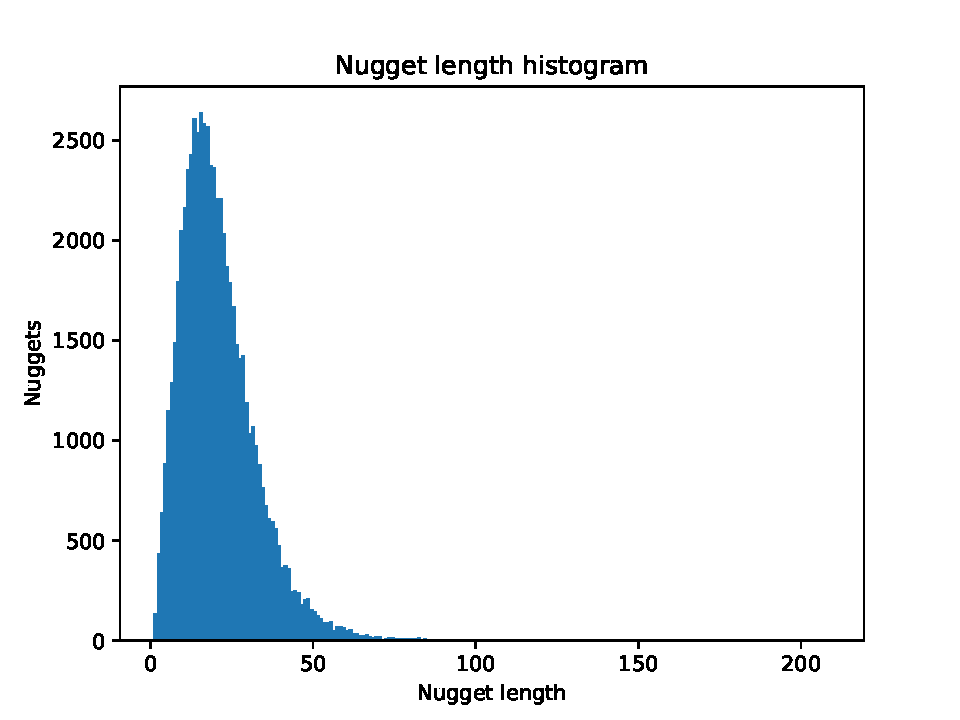
\includegraphics[width=0.55\linewidth]{Nugget_size.pdf}
	\caption{Nugget length distribution}
	\label{fig:nuggets}
\end{figure}
\ref{fig:nuggets}.
The results were that only about $49$ percent of the chosen nuggets are actual sentences and most of the nuggets are shorter than $15$ words.

\subsection{First approach}

For the first approach we chose to take a wordwise approach that was also inspired by problems additional to those mentioned above. The finding is that workers may choose different start or endpoints for nuggets leading to problems for approaches that would only consider nuggets important that match exactly for multiple workers. An example in our dataset for this can be found in table \ref{tab:nuggets}.
\begin{center}
	\begin{tabular}{ | l | p{7cm} |}
		\hline
		Worker ID & Nugget \\ \hline
		87b87beadeaabc197b466e265837af98 &  While some experts admit that neurofeedback has promise, they believe that it should be used only in combination with medication. \\ \hline
		f0a942943de19e11972338c883ad1da2 &  some experts admit that neurofeedback has promise, they believe that it should be used only in combination with medication. \\ \hline

		87954087f1d66c24165db6afc992e136 &  neurofeedback has promise, \\ \hline

		ec7e848297d5f2666f07c0d779ca074d	 &  neurofeedback has promise, they believe that it should be used only in combination with medication. \\
		\hline
	\end{tabular}
\label{tab:nuggets}
\end{center}
To avoid loss of such parts of sentences that are contained in multiple nuggets we therefore view each word of a sentence as a training / prediction instance. We do this by taking a word window with size $1$ around the particular word of interest which therefore contains the word and its left and right immediate neighbor. All those words are then transformed into word vectors from embeddings pretrained by Google\footnote{https://code.google.com/archive/p/word2vec/} and averaged. Similarily we also transform all words of the query of a specific topic into word embeddings and average them. In a third step both averages are averaged together once again to derive our word feature representation. We chose this final averaging step because we thought the arithmetic properties of word embeddings would retain information about the relation between word window and query. This also keeps the feature representation smaller than doing a concatenation for an example and therefore allowed us to still use classifiers that can not train on mini batches.

As labels each word got assigned a number which represents the amount of nuggets in the same sentence that contain that specific word. The different amounts of workers that chose a nugget then form the label of a classification task. A summarization of the process from a word of a sentence to feature representation can be found in pseudocode in  \ref{alg:features}. Here it is assumed that a sentence is padded accordingly.

\begin{algorithm}
	\label{alg:features}
	\SetKwInOut{Input}{input}

	\SetKwInOut{E}{E}
	\SetKwInOut{Output}{output}
	\SetKwInOut{QueryEmbedding}{QueryEmbedding}
	\SetKwInOut{WindowEmbedding}{WindowEmbedding}
	\SetKwInOut{SentenceWords}{SentenceWords}
	\SetKwInOut{QueryWords}{QueryWords}
	\E{Pre trained word embeddings}
	\QueryEmbedding{Averaged query embedding}
	\WindowEmbedding{Averaged word embedding of the word window}
	\SentenceWords{List of words in the sentence}
	\QueryWords{List of words in the query}

	\For{$i = 0;\ i < length(Query);\ i = i + 1$}{
		QueryEmbedding += Querywords[i]
	}
	QueryEmbedding /= length(Query)\;
	WindowEmbedding = E[SentenceWords[j-1]] + E[SentenceWords[j]] + E[SentenceWords[j+1]]\;
	WindowEmbedding /= 3\;


	return (QueryEmbedding+WindowEmbedding) /2 \;

	\caption{Feature building process}
\end{algorithm}


\begin{algorithm}
	\label{alg:the_alg}
	\SetKwInOut{Input}{input}
	\SetKwInOut{WordScore}{wordscore}
	\SetKwInOut{Classifier}{Classifier}
	\SetKwInOut{Output}{output}
	\SetKwInOut{Delta}{delta}
	\SetKwInOut{TempNugget}{tempNugget}
	\Input{List of words in a sentence}
	\Classifier{The trained word classifier}
	\WordScore{List of tuples containing word and their score}
	\Delta{The nugget word threshold}
	\TempNugget{List of words that form a nugget}
	\KwResult{List of Nuggets}
	\lForEach{word $w$ of input}{ wordscore.append($w$, Classifier(word)) }
	\For{(w, score) in wordscore}{
		\uIf{$score > delta$}{TempNugget.append(w)}
		\uElseIf{$score < delta$ and tempNugget not empty}{
			Result.append(TempNugget) \;
			TempNugget = empty list\;
		}
		\Else{
			skip\;
		}
	}
	return Result \;

	\caption{Nugget prediction process}
\end{algorithm}
To form nuggets in a sentence we first transform each word into the above described feature representation and then assign a class or score with the trained classifier. Afterwards nuggets are formed by concatenating consecutive words that have scores above a pre-defined threshold $\delta$. The whole process is defined in pseudocode in \ref{alg:the_alg}.

 \subsection{Second Approach}
For the second approach we used sequence classification to classify each possible subsequence of a sentence as either a nugget or not. More precisely we generated a candidate $s_{i,m}=(w_i, w_{i+1}, \dots , w_{i+m})$ for each word $w_i$ with $m$ following words. We iterated the candidate length $m=|s_{i,m}|$ between a minimum length of 5 and a maximum of 20, if the length of the sentence allowed it. So $5 \leq m \leq 20$. In the end we would have every possible candidate in any given sentence. \\
This preprocessing required substantive computational time, so we saved these candidates to the disk to have the whole training set availabe and speed up the training process. We found that only a few percent of possible nugget candidates actually were annotated by at least one worker. This extreme class imbalance can lead to serious issues in the learning process with most models \cite{japkowicz2002class}. To fix this issue we used oversampling of the rare class, i.e. after shuffling all samples we would take 20\% candidates with a label bigger than zero and 80\% random candidates. This makes it much more likely to have at least one positive sample in each batch, so that the model can have a more stable training signal.

We chose this approach because it seems like an intuitive solution to the problem that nuggets can also be incomplete sentences. In many of the target nuggets we were given, the workers annotated only the most important phrases of a sentence.

To represent the nugget candidates we used sequences of pretrained Word2Vec word embeddings \cite{w2v}, as well as sentence embeddings computed by the Universal Sentence Encoder module in tensorflow \cite{universal2018}. Since the generation of the sentence embeddings took very long, we were unable to generate them for the whole training set and did not include them in the final architecture. Additionally we used the word embeddings of the query sequence as an additional input.

To identify the correct nuggets we could use classification with two classes: nugget or not a nugget. This makes the task similar to sentence classification, which is a very well researched problem. The difference is that nuggets can be incomplete sentences. As \citep{zhou2015c} and others have shown, RNNs are among the top performing models in sentence classification together with CNNs, if given enough training data. For the target data we used a threshold of two, so any phrase which was annotated as a nugget by two or more workers would be considered a nugget in this binary format. Also possible would be regression of the number of Mechanical Turk workers annotating each word sequence as a nugget. Which would be equivalent to the original format of our target data.\\

\begin{figure}
\begin{tikzcd}
\label{fig:2nd_regression}
query \arrow[rd, "embedding"] &  &  &  \\
 & {GRU(256, relu)} \arrow[r] & {Dense(256,relu)} \arrow[r] & {Dense(1, linear) MSE} \\
sequence \arrow[ru, "embedding"'] &  &  & \\
\end{tikzcd}
\caption{Architecture of the second approach with regression}
\end{figure}

All put together we used the architecture as shown in figure \ref{fig:2nd_regression} for regression. Similarily for classification we used binary labels, softmax and crossentropy loss.
We used GRUs as proposed by \cite{gru2014}, because we have less training data than most state of the art research projects. While the performance of LSTMs and GRUs are very similar, the GRU has a bit fewer parameters to train and is thus less computationally demanding and easier to generalize \cite{cnn_rnn_comparative2017}. We also tried a similar architecture for classification of candidates with more than one worker annotating it. Sadly both architectures did not learn anything beyond always predicting 0, i.e. no nugget. We tried different models in order to find the problem, but we were uable to improve the model significantly. Perhaps the class imbalance was still too high or we made a mistake selecting the nugget candidates and corresponding labels. In the end we sadly had to abandon the approach in favor of the first one, so we also don't discuss resulting nuggets of the second approach in the later sections.


\subsection{Generating summaries}
Since the ultimate goal of the project was to generate summaries. As suggested by the advisors we chose to collaborate with group $5$. Their pipeline required exactly 30 sentences per topic sorted by their importance for the summary. As our approaches did not necessarily lead to sentence outputs we had to come up with a workaround to fulfill the necessary requirements.  

We eventually decided to proceed the following way. For every sentence of a topic we calculate the percentage of words that appear in nuggets chosen by our model. Sentences that have a percentage smaller than $40$ percent are excluded. Afterwards we gave group $5$ our top $30$ sentences with regards to words in a nugget in descending order and then received their final model output which is further evaluated in \ref{subsec:maneval}.   
\section{Evaluation}
\label{sec:eval}

\subsection{Nugget Evaluation}
We tried to evaluate both our main approaches on the labeled dataset \cite{Tauchmann.et.al.2018.LREC}. Since the second approach did not learn anything we abandoned it for the final predictions and also do not report performance measures in the following chapters. For the evaluation of the first approach we chose $2$ out of the $10$ labeled topics and split them into one development set topic and a test set topic respectively. As for all the machine learning models we use the popular scikit-learn python module. Since our computational resources were limited we only were able to test three different models in a reasonable timeframe such as Decision trees, logistic Regression and Random forests. For the latter training however took significantly longer than for the other two so less hyperparameters were tested.
The final scores on the Test set can be found in table \ref{Nugget_scores}.
\begin{table}
	\caption{Nugget Evaluation Scores}
	\label{Nugget_scores}
	\centering
	\begin{tabular}{llll}
		\toprule
		\multicolumn{4}{c}{}                   \\

		Model     & Recall & Precision & F1 \\
		\midrule
		DecisionTree & $0.901$  & $0.1501$ &   $0.257$   \\
		RandomForest     & $0.887$ & $0.137$ &   $0.237$   \\
		LogisticRegression     &  $0.891$ & $0.09$ & $0.163$  \\
		\bottomrule
	\end{tabular}
\end{table}

\subsubsection{Nugget results discussion}
The overall performance of the nugget selection were quite disappointing and can have many different causes. One obvious factor is the relatively unorthodox selection of nuggets which is evident in the high recall scores. This happened mainly because we had to set the threshold of nuggets to $1$ as otherwise no nuggets would have been predicted. We tried to sum class probabilities and modeling the task as regression but the heavy imbalance between label values always led to similar problems in the results. A bigger dataset would have allowed us by the means of subsampling to provide a more balanced class distribution and therefore possibly achieve better results. Also the query or topic should be a rather important information about what is might be a nugget in a sentence. The provided labeled dataset only has ten such topics though which might also not be enough data to allow for a generalizable solution in the first place.  However it may also be concluded that the chosen feature representation due to the averaging or relatively narrow view on the sentence does not provide a clear enough boundary between important and unimportant words/nuggets.

To address the unclear effect of this feature representation we originally thought about using our second approach which however failed as well. We mainly guess that it was due to a lack of annotated data as it was easy to create vast amount of negative labeled nuggets but the relatively limited amount of queries and annotated nuggets might be problematic for learning a decently sized recurrent neural network. Another possibility is that the labels were not continous enough between sentences. Two sentences which only differ by one word often have completely different labels, because we annotated only the exact sequence. This may lead to a almost flat error surface where the only positive areas are distributed more by chance than by correlation with the sequence's embeddings. As an example we think the addition of sequence similarity between wrong and nearby true nuggets could help achieve a more stable training signal towards target sequences.
\subsection{Automatic Evaluation}
For the automatic evaluation of our generated summaries we use Rouge-2 and Jensen Shannon divergence(JSD). JSD does not require gold standard reference summaries and therefore is easily computed on our output. Rouge Scores however typically depend on reference summaries which required us to provide those references by treating summaries of other groups as such. 

\subfile{sections/rouge}

\subsubsection{Jenson Shannon Divergence}
The final results for unsmoothed and smoothed JSD can be seen in table \ref{tab:jensen}

\begin{table}
	\caption{Jensen Shannon divergence scores}
	\label{tab:jensen}
	\centering
	\begin{tabular}{llll}
		\toprule
		\multicolumn{3}{c}{}                   \\
		
		Model     & Smoothed JSD & Unsmoothed JSD \\
		\midrule
		Baseline 1 & $0.292$  & $0.515$ \\
		Our Output     & $0.290$ & $0.517$    \\
		Average all groups & $0.275$& $0.495$ \\
		\bottomrule
	\end{tabular}
\end{table}

The results show that our group performs roughly on par with the baseline provided by the course instructors while being slightly outperformed by the rest of course groups. This also was to be expected as mentioned in \ref{sec:eval} our system had problems where it would frequently mistake irrelevant information as nuggets.
\subsection{Evaluation of manual evaluations}
\label{subsec:maneval}
\subfile{sections/manual_evaluations}

\subfile{sections/conclusion}
\subfile{sections/future_work}

\bibliographystyle{plain}
\bibliography{nips_2018}


\end{document}
